\chapter{Implementation}
\label{chap:Chapter 4 title}
\section{Introduction}

The implementation chapter is a crucial step in our project. In this chapter, we will present in detail the various steps we followed to implement our solution. Overall, this implementation chapter will allow us to document in a detailed and transparent manner the process of executing our project. It will highlight the efforts made, the choices made, and the results obtained.

\pagebreak

\section{Configuration \& Deployment}
\subsection{Creating a GitLab Template for Kepler}

To successfully integrate Kepler with our GitLab CI pipeline and ensure a seamless, efficient, and automated workflow, we followed a series of steps that included configuring the necessary environments, creating precise configuration files, and integrating essential monitoring tools
\subsection*{Configuration of the Environment}

The initial step was to set up the execution environment for GitLab CI. We configured the runners, which are the virtual machines or containers responsible for executing the CI jobs. It was crucial to ensure that all dependencies required to run Kepler, Prometheus, and Grafana were installed on these runners.

\subsection*{Creation of the CI Configuration File}

We added a \texttt{template-ci-kepler.yml} file. This file plays a 
role as it defines the various stages of the CI pipeline and specifies the actions required to integrate Kepler into our CI process. By using this configuration file, we were able to clearly and systematically outline the tasks necessary for seamless integration into our pipeline.

 \begin{figure}[H]
    \centering
    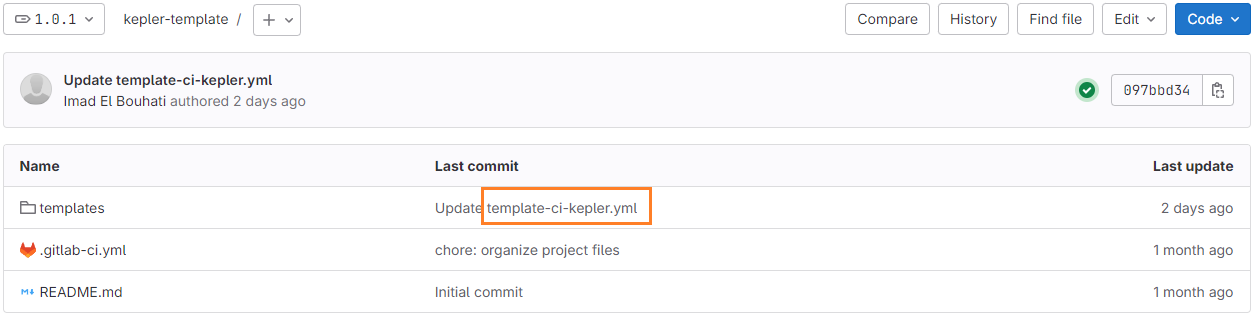
\includegraphics[width=19cm]{Figures/kepler-template-gitlab.png}
    \caption{Kepler template repository}
\end{figure}

\subsection*{Integration of the Kepler Template}

After creating the template, it can be used and integrated directly into a project. To achieve this, a few lines must be added to the \texttt{.gitlab-ci.yml} file.

First, we add the \texttt{include} directive followed by the path to our directory containing the Kepler template into an existing pipeline.

\begin{figure}[H]
  \centering
  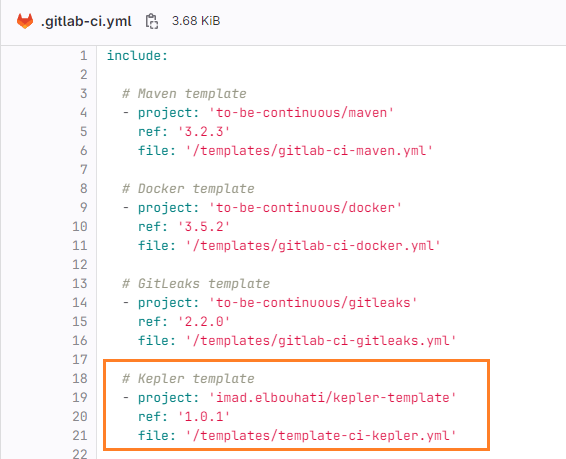
\includegraphics[width=13cm]{Figures/kepler-template-integration.png}
  \caption{Integration of the Kepler template}
\end{figure}

Next, we specify the stage name as \texttt{"deploy"}.

\begin{figure}[H]
  \centering
  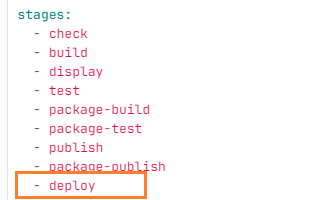
\includegraphics[width=10cm]{Figures/deploy-kepler-stage.png}
  \caption{Stage \texttt{"deploy"}}
\end{figure}

We define the following variables for the deployment:

\begin{itemize}
    \item \texttt{HELM\_RELEASE\_NAME} as the name of our Helm release.
    \item \texttt{HELM\_NAMESPACE} as the namespace for our Helm deployment.
    \item \texttt{KUBECONFIG\_CONTENT} to store cluster authentication information for kubectl.
\end{itemize}

\begin{figure}[H]
  \centering
  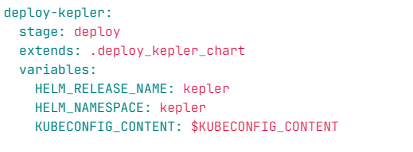
\includegraphics[width=0.8\textwidth]{Figures/deployment-variable.png}
  \caption{Deployment variables for Kepler}
\end{figure}

This configuration allows us to include the steps for deploying Kepler in our CI/CD pipeline using Helm and Kubernetes.


\subsection{Deploying Prometheus \& Grafana on Kubernetes}

To deploy Prometheus and Grafana in our Kubernetes cluster as part of the existing CI/CD pipeline, we have followed a structured approach. This ensures that both monitoring and visualization tools are set up correctly and efficiently.

First, we create a new job in the \texttt{.gitlab-ci.yml} file named \texttt{deploy-prometheus-grafana}. This job will run after the \texttt{deploy-kepler} job, ensuring that Kepler is deployed before Prometheus and Grafana.

\begin{figure}[H]
  \centering
  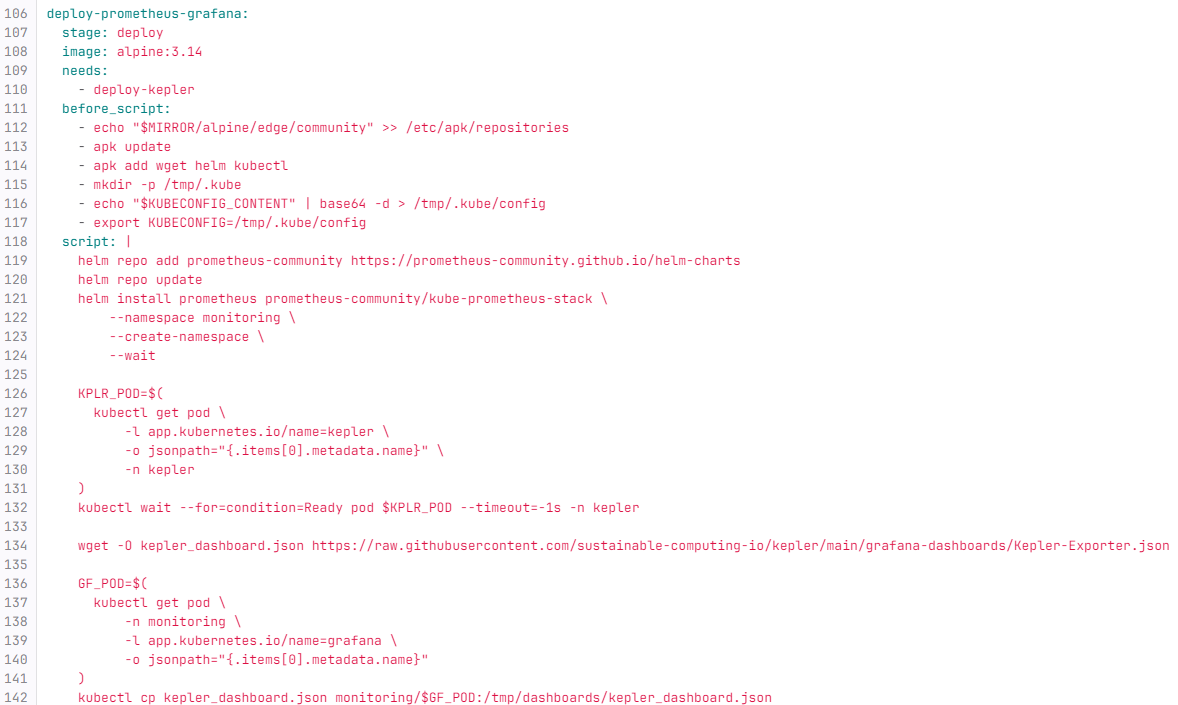
\includegraphics[width=16cm]{Figures/deploy-prometheus-grafana-job.png}
  \caption{Job \texttt{deploy-prometheus-grafana}}
\end{figure}

Next, we define the necessary configurations and scripts for deploying Prometheus and Grafana.
This script accomplishes the following:

\begin{itemize}
  \item Adds the Prometheus Helm chart repository and updates Helm repositories.
  \item Installs the Prometheus stack in the \texttt{monitoring} namespace.
  \item Waits for the Kepler pod to be ready.
  \item Downloads the Kepler Grafana dashboard JSON file.
  \item Finds the Grafana pod and copies the Kepler dashboard JSON file to it.
\end{itemize}

\subsection{Configuring Rules and Alerts in Prometheus}
In this section, we will cover the steps involved in configuring Prometheus to monitor specific metrics and set up alerting rules to notify us of any anomalies. Prometheus allows us to define custom rules for generating alerts based on our metrics, which can be integrated with various notification channels like Slack.

\subsubsection{Creating Custom Alerting Rules}

To monitor the energy consumption of our nodes, we have defined several custom alerting rules. These rules are specified in the \texttt{additionalPrometheusRulesMap} section of our Prometheus configuration. Here is an example configuration:

\begin{figure}[H]
    \centering
    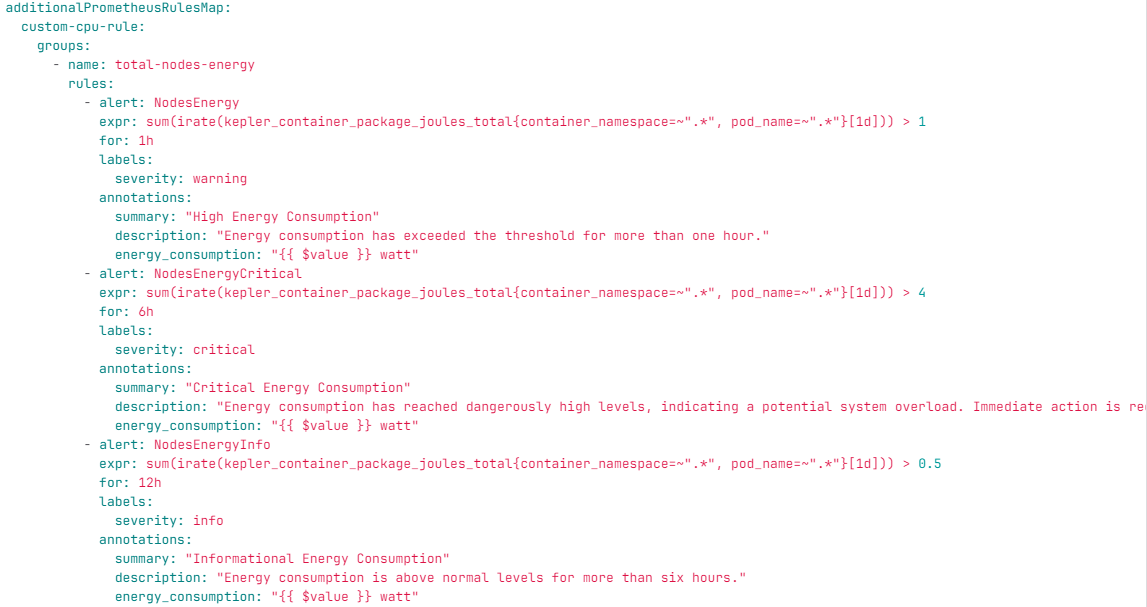
\includegraphics[width=16cm]{Figures/prometheus-rule.png}
    \caption{Prometheus rules}
\end{figure}

This configuration defines three alerts:

\begin{itemize}
  \item \textbf{NodesEnergy}: Triggered when the energy consumption exceeds 1 watt for more than 1 hour. It has a \texttt{severity} label set to \texttt{warning}.
  \item \textbf{NodesEnergyCritical}: Triggered when the energy consumption exceeds 4 watts for more than 6 hours. It has a \texttt{severity} label set to \texttt{critical}.
  \item \textbf{NodesEnergyInfo}: Triggered when the energy consumption exceeds 0.5 watts for more than 12 hours. It has a \texttt{severity} label set to \texttt{info}.
\end{itemize}

Each alert includes annotations providing a summary and description of the alert, along with the actual energy consumption value.

\begin{figure}[H]
  \centering
  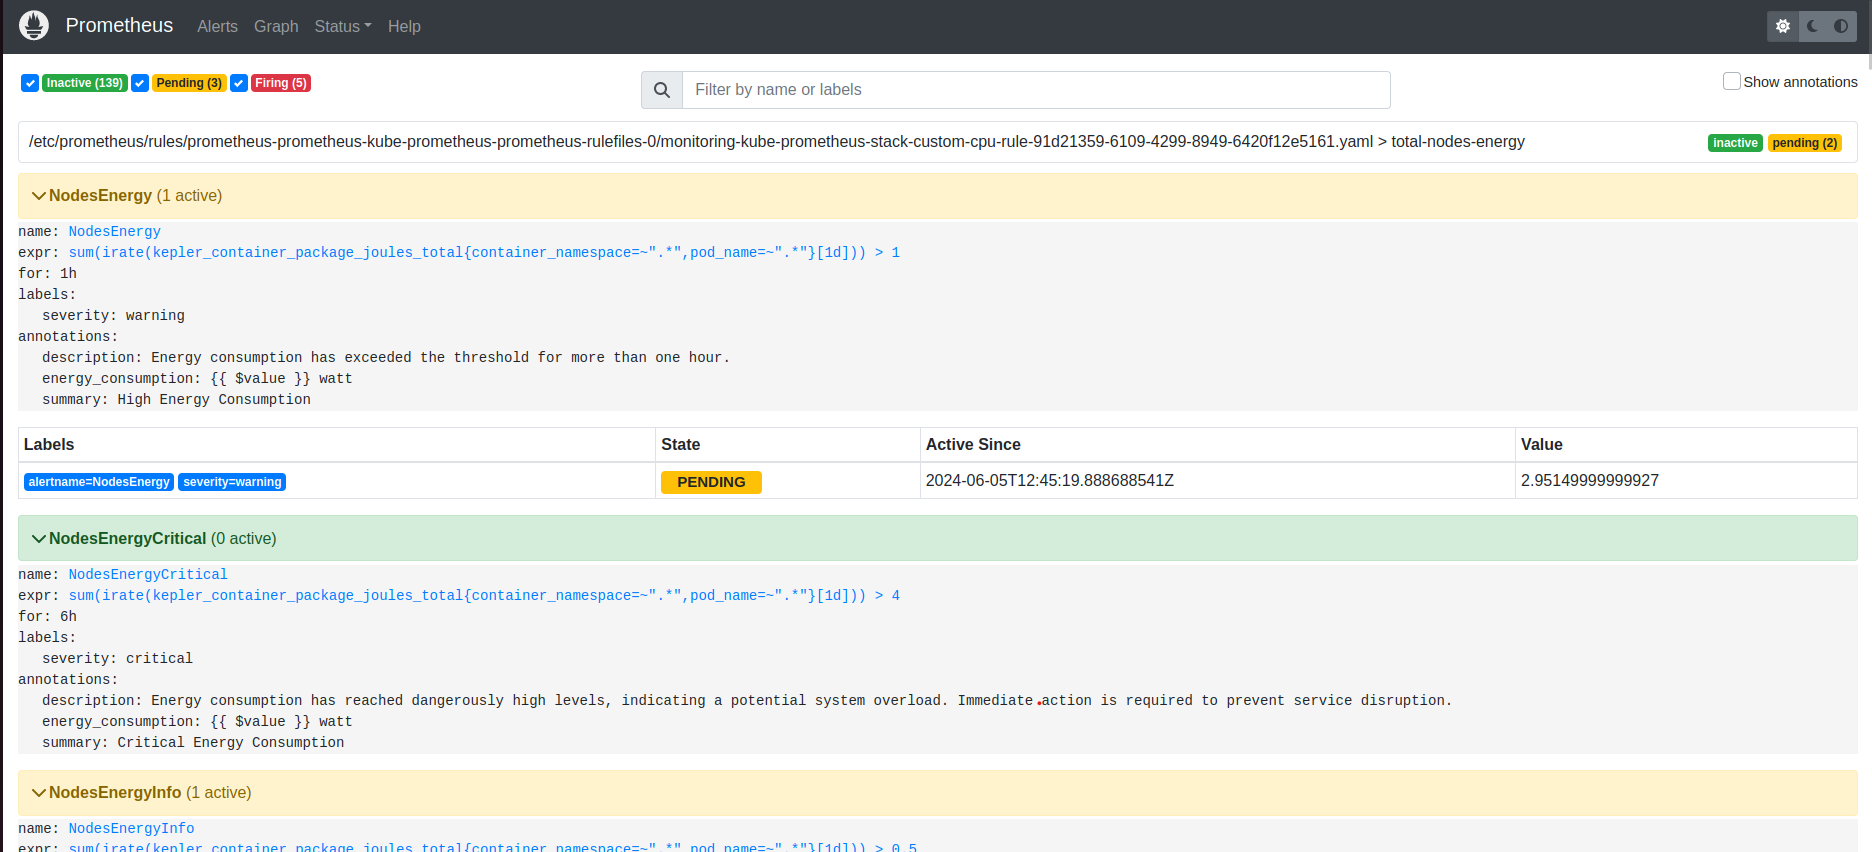
\includegraphics[width=0.8\textwidth]{Figures/alerts.png}
  \caption{Alerts dashboard in Prometheus}
\end{figure}

\subsubsection{Integrating Alerts with Slack}

To ensure that we receive notifications for these alerts, we integrate Prometheus with Slack using Alertmanager. The following configuration sets up Alertmanager to send alerts to a Slack channel:

\begin{figure}[H]
    \centering
    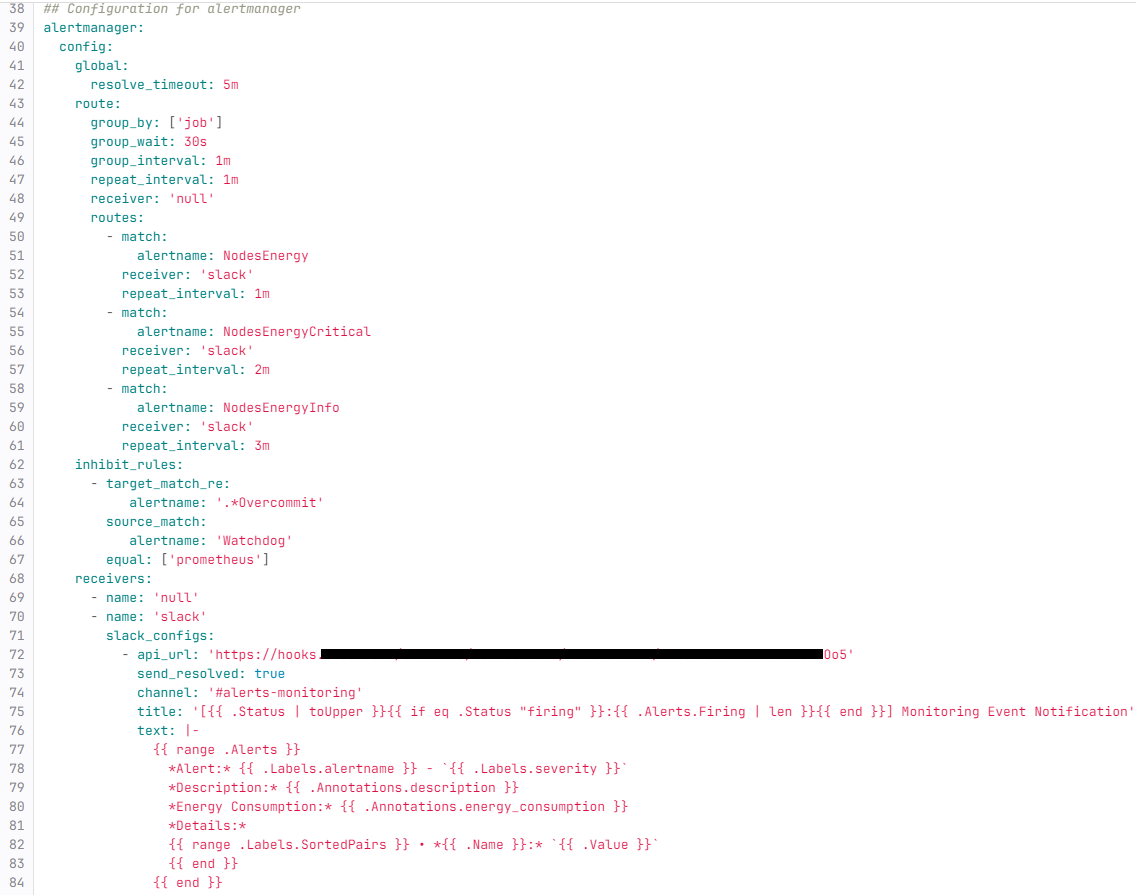
\includegraphics[width=0.8\textwidth]{Figures/alert-manager.png}
    \caption{Alert Manager Configuration}
  \end{figure}

This configuration does the following:

\begin{itemize}
  \item Sets global configuration options such as \texttt{resolve\_timeout}.
  \item Defines routing rules to determine which alerts should be sent to Slack. Alerts named \texttt{NodesEnergy}, \texttt{NodesEnergyCritical}, and \texttt{NodesEnergyInfo} are routed to the Slack receiver.
  \item Sets up inhibition rules to prevent redundant alerts.
  \item Configures the Slack receiver with a webhook URL, ensuring that alerts are sent to the \\
  \texttt{\#alerts-monitoring} channel. The \texttt{title} and \texttt{text} fields format the alert message.
\end{itemize}

\begin{figure}[H]
  \centering
  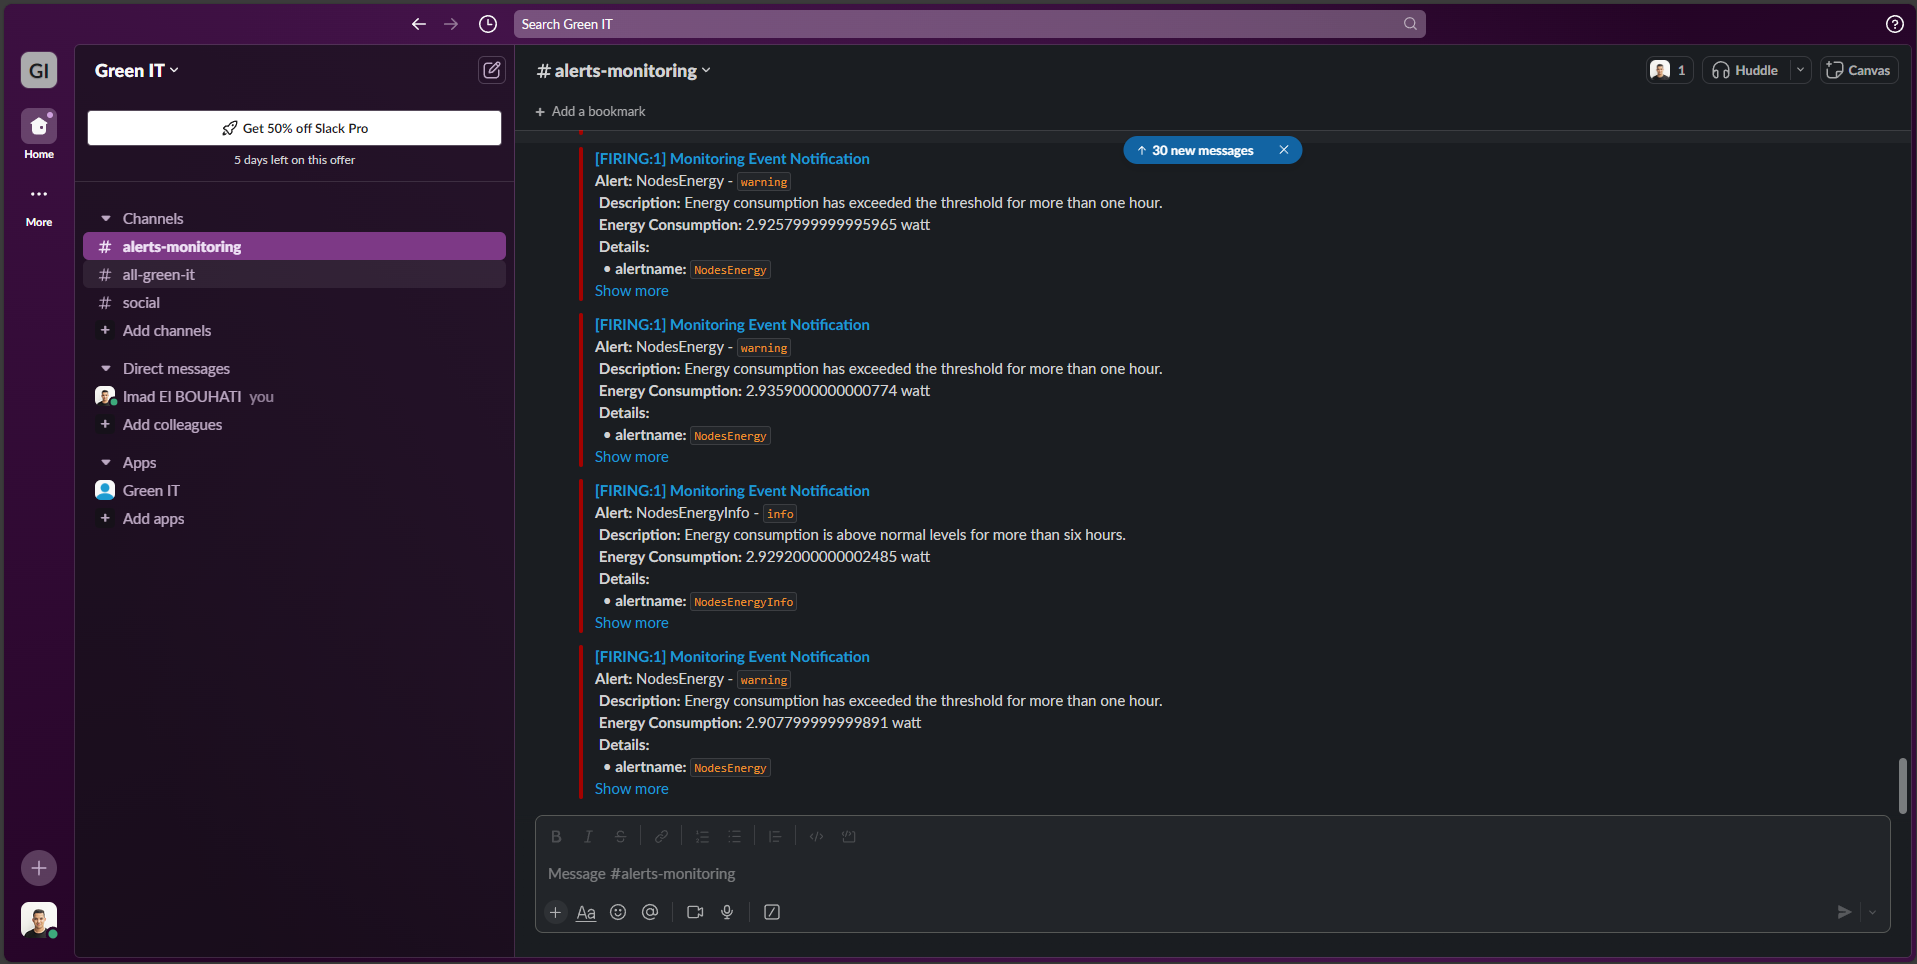
\includegraphics[width=0.8\textwidth]{Figures/slack-green-it channel.png}
  \caption{Slack alerts messages}
\end{figure}

\section{Launching the CI/CD Pipeline}

In this section, we will discuss the process of launching our CI/CD pipeline, showcasing the various stages and the resources deployed in our Kubernetes cluster. Finally, we will present the Grafana dashboard to visualize the metrics collected by Prometheus.

\subsection{Starting the GitLab Pipeline}

To start the pipeline, we push our code changes to the GitLab repository. This triggers the GitLab CI/CD pipeline, which executes the stages defined in the \texttt{.gitlab-ci.yml} file. The pipeline consists of multiple stages, including building, testing, and deploying our applications.

\begin{figure}[H]
  \centering
  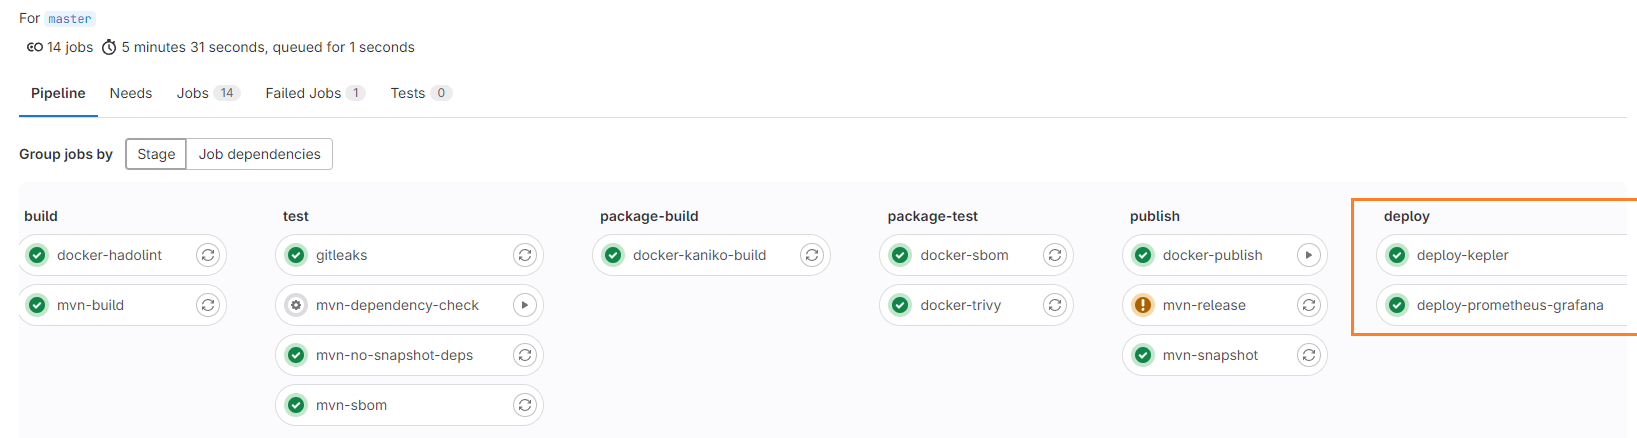
\includegraphics[width=0.8\textwidth]{Figures/gitlab-pipeline.png}
  \caption{GitLab CI/CD Pipeline Stages}
\end{figure}

\subsection{Deployed Resources in Kubernetes}

Once the pipeline completes successfully, the following resources were deployed in the `kepler` and `monitoring` namespaces within our Kubernetes cluster.

\subsubsection{Kepler Namespace}

The `kepler` namespace contains the resources related to the Kepler application. These resources include:

\begin{itemize}
    \item \textbf{Pod}: The running instance of the Kepler application.
    \item \textbf{Service}: Provides a stable IP and DNS name for accessing the Kepler application.
    \item \textbf{DaemonSet}: Ensures that a copy of the Kepler application runs on all nodes.
\end{itemize}

\begin{figure}[H]
    \centering
    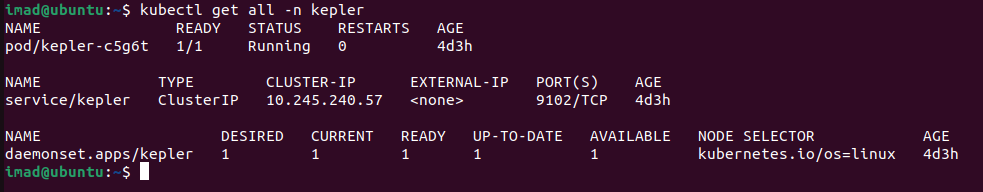
\includegraphics[width=\linewidth]{Figures/kepler-monitoring-resources.png}
    \caption{Deployed resources in the `kepler` namespace.}
    \label{fig:kepler-resources}
\end{figure}

\subsubsection{Monitoring Namespace}

The `monitoring` namespace contains the resources for monitoring and alerting. These resources include:

\begin{itemize}
    \item \textbf{Prometheus}: Collects and stores metrics data.
    \item \textbf{Alertmanager}: Manages alerts sent by Prometheus.
    \item \textbf{Grafana}: Visualizes the collected metrics.
    \item \textbf{Services}: Provide stable IPs and DNS names for accessing Prometheus, Alertmanager, and Grafana.
    \item \textbf{DaemonSet and Deployments}: Ensure that Prometheus and its components are running correctly.
\end{itemize}

\begin{figure}[H]
    \centering
    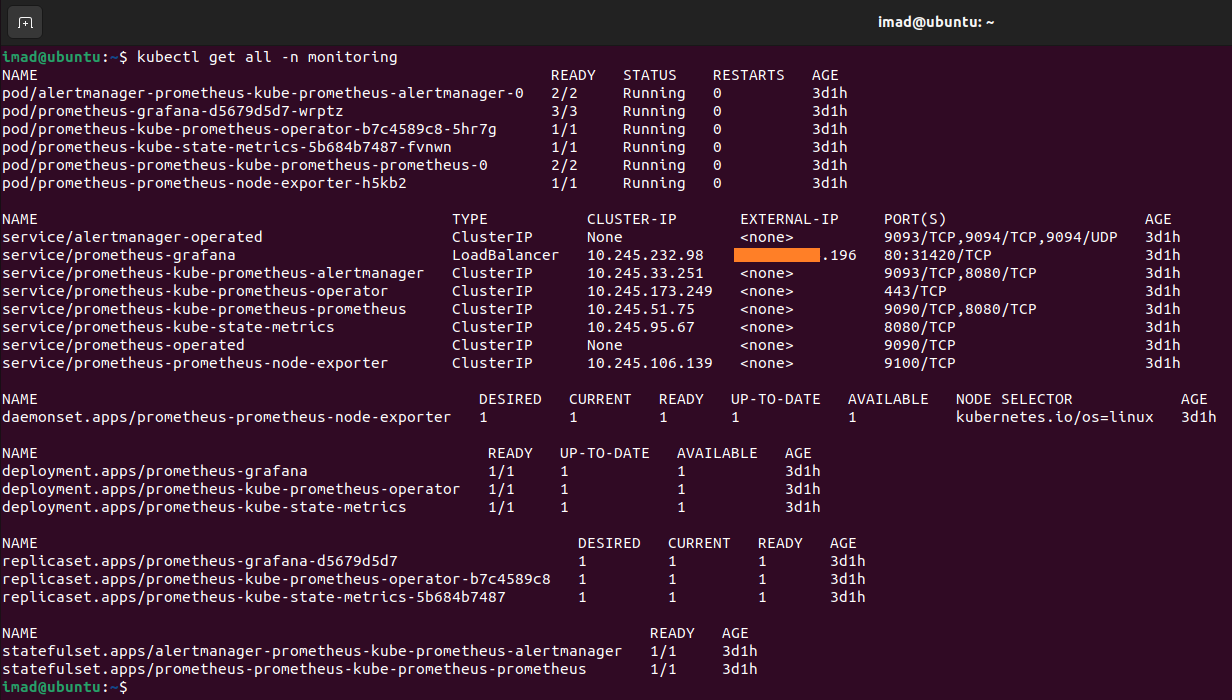
\includegraphics[width=\linewidth]{Figures/monitoring-namespace-resources.png}
    \caption{Deployed resources in the `monitoring` namespace.}
    \label{fig:monitoring-resources}
\end{figure}

\subsection{Grafana Dashboards}
We utilize Grafana dashboards to monitor the performance and resource utilization of our Kubernetes cluster. Below are the key metrics visualized:
\subsubsection{Carbon Emissions Dashboard}
\begin{figure}[H]
    \centering
    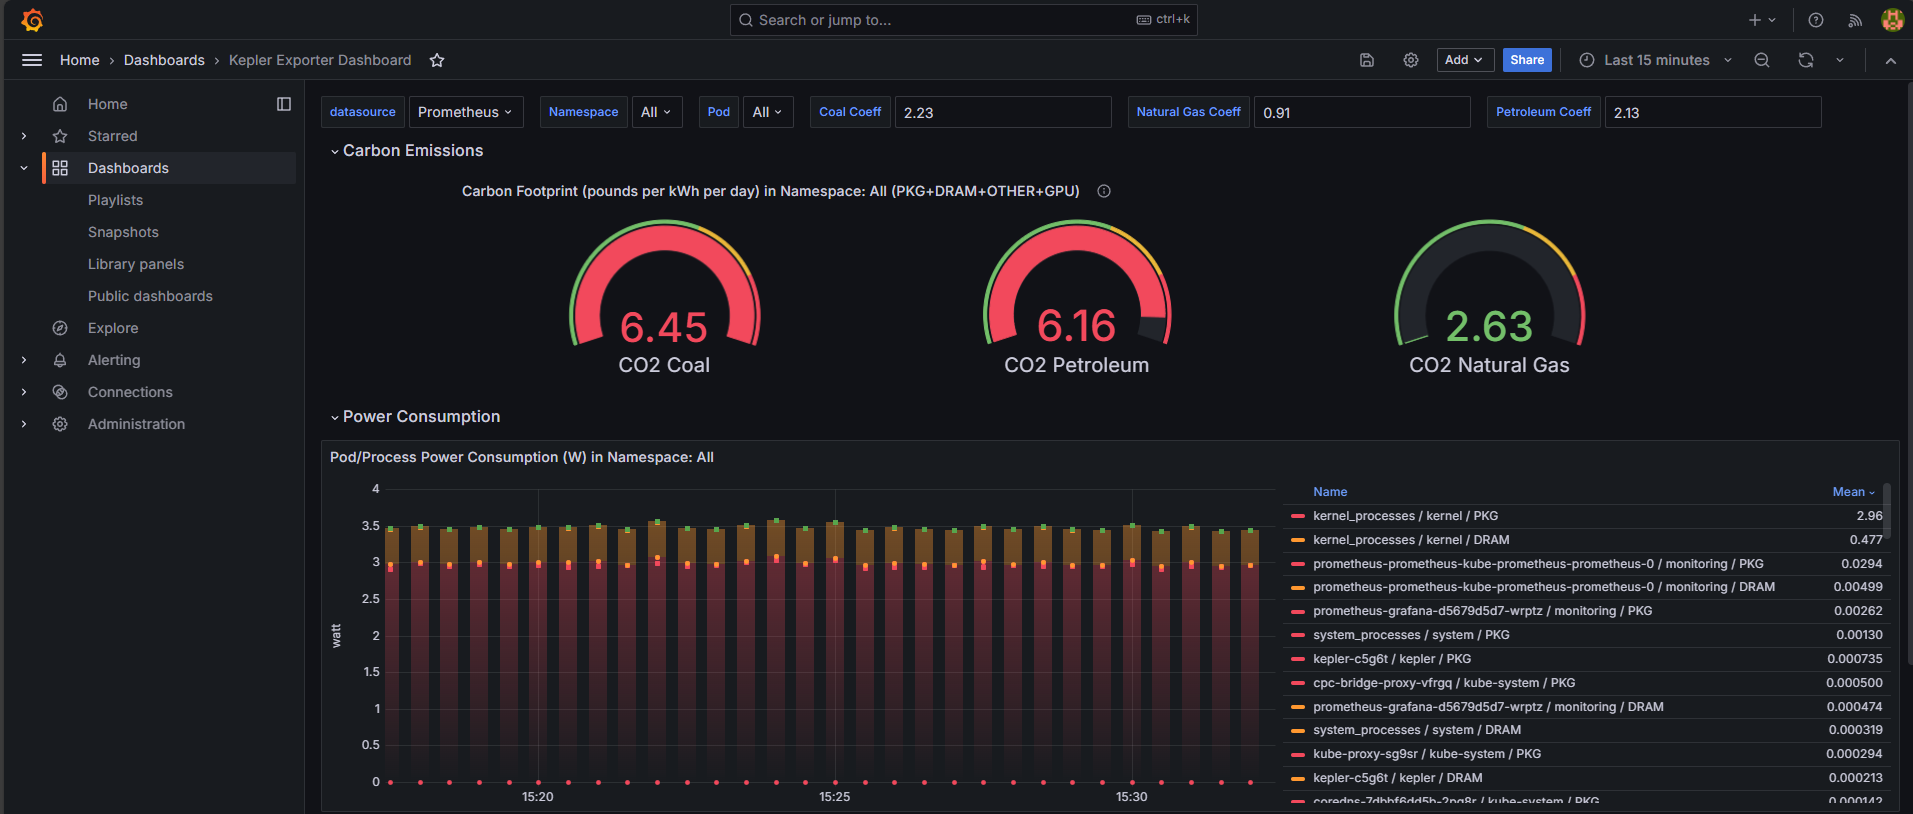
\includegraphics[width=\textwidth]{Figures/grafana-dashboard-1.png}
    \caption{Grafana dashboard showing carbon emissions based on energy consumption.}
    \label{fig:grafana-dashboard-2}
\end{figure}

The above figure (Figure \ref{fig:grafana-dashboard-2}) shows the carbon emissions associated with the energy consumption in the cluster. The dashboard highlights the carbon footprint in terms of \texttt{CO$_2$ Coal}, \texttt{CO$_2$ Petroleum}, and \texttt{CO$_2$ Natural Gas}. This information is crucial for understanding the environmental impact of our infrastructure and taking steps towards sustainability.


\subsubsection{Power Consumption Dashboard}
\begin{figure}[H]
    \centering
    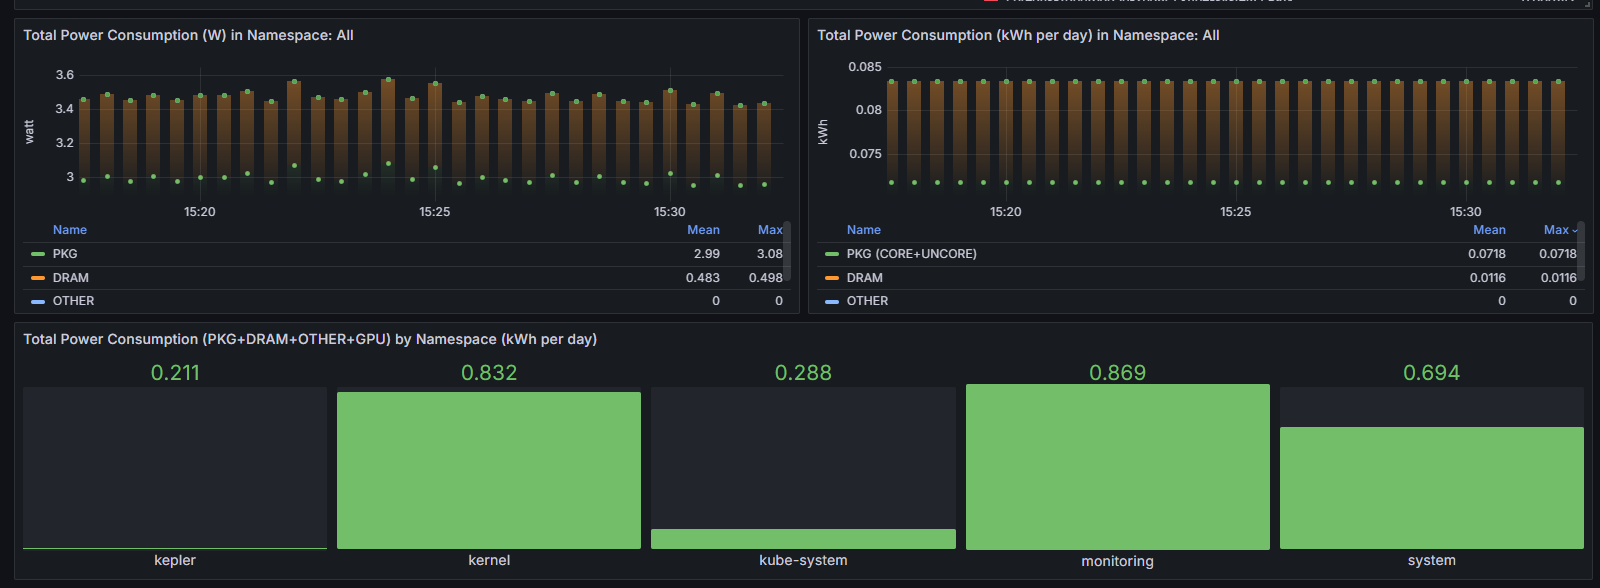
\includegraphics[width=\textwidth]{Figures/grafana-dashboard-2.png}
    \caption{Grafana dashboard showing total power consumption by namespace.}
    \label{fig:grafana-dashboard-1}
\end{figure}

The above figure (Figure \ref{fig:grafana-dashboard-1}) displays the total power consumption (in watts) across all namespaces in the cluster. The power consumption is broken down into different components: \texttt{PKG} (Package), \texttt{DRAM} (Memory), and \texttt{OTHER}. The dashboard provides insights into the energy usage trends over time, which helps in optimizing resource allocation and identifying potential inefficiencies.



\newpage

\section{Conclusion}

Integrating our CI/CD pipeline with Kubernetes and monitoring tools has enabled efficient deployment and management of large-scale resources. The \texttt{kepler} and \texttt{monitoring} namespaces hosted essential pods, services, and daemons, ensuring high availability and simplified maintenance.
The Grafana dashboards provide detailed views of power consumption and CO$_2$ emissions, facilitating proactive and sustainable infrastructure management. This approach not only optimized performance but also helped minimize the environmental impact of our operations.
Future improvements could include integrating additional monitoring features and extending our CI/CD pipeline with complementary tools to enhance the robustness and security of our Kubernetes ecosystem.

\pagebreak